\section{Feasibility experiments}
\label{sec:feasibility}
To gauge the feasibility of the proposed graduation project several aspects of the Lightyear 0 were researched and some experiments with tools were performed. This section describes how the research and experiments were performed and the resulting models, descriptions and data of the experiments.

Section~\ref{sec:invehicle} describes the architecture of the Lightyear 0's in-vehicle network, explaining the different types of nodes found in the network, which networks the vehicle has and the connections between component and network. The results were created by both talking to experts on the in-vehicle network, reading documentation and reading code that is deployed on the nodes or used to build the binaries. 
Section~\ref{sec:networktraffic} is an investigation into the data that is generated and consumed by the nodes in the network. The goal is to understand what kinds of dataflows exist in the Lightyear 0 so that the network traffic produced by these flows can be modelled accurately during the graduation project. The execution model of the node types mentioned in Section~\ref{sec:invehicle} is described as well to make the dataflow model more accurate. Some scripts have been developed to partially retrieve and generate overviews of the dataflow from the program code. This section is a result of inspecting the build-system and the code that is deployed on the network nodes, followed by a review by the architects and lead software developers of the system.

Lastly in Section~\ref{sec:omnetpp} an experiment performed with the Discrete Event Simulator \omnet is explained. The experiment is a re-implementation of an exercise performed during the \textit{Quantitative Evaluation of Embedded Systems} course which was originally executed in Matlab. The goal is to learn the basics of the simulation framework and validate its ability to perform experiments involving random processes.

\subsection{The in-vehicle network}
\label{sec:invehicle}
The Lightyear 0's in-vehicle network is based on a decentralized domain architecture, with CAN and LIN as the main network technologies with Ethernet being used for non-real time applications. Meaning that networked components pertaining to the same function or domain (body control, powertrain etc.) are grouped together in a network. The networks are linked together using a central gateway who is responsible for bridging necessary data between networks. For example information about the motor power might be required in the Battery Management System, Propulsion Controller and Media Controller. But for various reasons these controllers might not all be connected to the same network, so the motor power information needs to be forwarded on the relevant networks.

At the core of the embedded system are three ECUs named the Central Gateway, Vehicle Control Unit and Safety Control Unit. The Safety Control Unit contains two heterogeneous cores, that both have access to the connected CAN busses. Each ECU has a real-time operating system (RTOS) with a rate monotonic preemptive scheduler and can be connected up to four CAN busses and two LIN busses. The software on these ECUs is developed by Lightyear and thus the functionality of an ECU is not fixed or prescribed by a vendor. As the functionality is not fixed we will call these ECUs \textit{programmable end nodes} for modelling purposes.

The other nodes in the network have a fixed function, some of them are developed by Lightyear such as motor inverters and solar converters, while others are developed by third parties. Some of these nodes can be configured by the user to tune the behaviour, while others are completely fixed. In some cases the parameters that can be changed are related to the network behaviour e.g., changing the CAN identifiers of certain messages. For ease of modelling we call these fixed function nodes \textit{parametrizable end nodes}, even if a node is completely fixed and cannot be configured. The inner workings of parametrizable end nodes varies and is often unknown in case of third party components. Fortunately the only necessary knowledge for an accurate network simulation is the external behaviour. Because parametrizable end nodes must be integrated, a precise specification of the network traffic generated and consumed by the end node is available and can be used for modelling purposes.

Three special cases of parametrizable end nodes are worth mentioning, the motor inverters (inverter), the media ECU and the telematics control unit. The motor inverters and media ECU have both a CAN interface and Ethernet interface. The telematics control unit has a CAN interface, Ethernet interface and a wireless modem, giving access to the internet which is shared with the media ECU so that applications such as navigation can use online services.

Table~\ref{tab:networks} gives an overview of all the networks in the car and which nodes are connected to which bus. For brevity a subset of the \textit{parametrizable end nodes} is enumerated, it can be assumed that each bus has several extra nodes connected. Information of the not mentioned nodes is available but simply left out for space reasons. The two LIN busses, LIN A and LIN B, each connect to the Central Gateway which acts as the master in the LIN networks. The slave nodes are third party off the shelf components and can be classified as \textit{parametrizable end nodes}. The same information is represented in diagram form in Figure~\ref{fig:networkoverview}.

Finally, there are components in the vehicle that generate or consume data but are not seen as a networked component in the "traditional" sense. Examples of such components are speakers, which consume audio data, rearview cameras which produce image data, instrument cluster displays which consume video/graphical data. Further investigation is necessary to determine how many of these nodes exist, how they are connected and how they should be modelled from a networking perspective.

\begin{table}[htb]
    \centering
    \resizebox{\textwidth}{!}{%
    \begin{tabular}{@{}lllllllllllllllllll@{}}
                                & \multicolumn{10}{c}{Controller Area Network} & \multicolumn{2}{c|}{LIN} & \multicolumn{5}{c}{Ethernet} & \multicolumn{1}{c}{Other} \\* \cmidrule(lr){2-11} \cmidrule(r){12-13} \cmidrule(r){14-18} \cmidrule(r){19-19}
    Node name                & \multicolumn{1}{R{2.5cm}}{Driver support} & \multicolumn{1}{R{2cm}}{Drivetrain} & \multicolumn{1}{R{2cm}}{Energy\\ management} & \multicolumn{1}{R{2cm}}{HVBS} & \multicolumn{1}{R{2cm}}{Powertrain} & \multicolumn{1}{R{2cm}}{Solar} & \multicolumn{1}{R{2cm}}{Surrounding\\ sense} & \multicolumn{1}{R{2cm}}{Telematics} & \multicolumn{1}{R{2cm}}{Vehicle} & \multicolumn{1}{R{2cm}}{Vehicle 2} & \multicolumn{1}{R{2cm}}{LIN A} & \multicolumn{1}{R{2cm}|}{LIN B} & \multicolumn{1}{R{2cm}}{Media} & \multicolumn{1}{R{2cm}}{Inverter FL} & \multicolumn{1}{R{2cm}}{Inverter FR} & \multicolumn{1}{R{2cm}}{Inverter RL} & \multicolumn{1}{R{2cm}}{Inverter RR} & \multicolumn{1}{R{2cm}}{Others}   \\*\cmidrule(r){1-1} \cmidrule(r){2-11}\cmidrule(r){12-13} \cmidrule(r){14-18} \cmidrule(r){19-19}
    Vehicle Control Unit     & X &   &   &   &   & X & X &   & X &   &   & \multicolumn{1}{c|}{}  &   &   &   &   &   &   \\
    Central Gateway          &   &   &   &   & X &   &   & X & X & X & X & \multicolumn{1}{c|}{X} &   &   &   &   &   &   \\
    Safety Control Unit      &   & X & X & X & X &   &   &   &   &   &   & \multicolumn{1}{c|}{}  &   &   &   &   &   &   \\
    Steering Column Module   & X &   &   &   &   &   &   &   &   &   &   & \multicolumn{1}{c|}{}  &   &   &   &   &   &   \\
    Inverter FL              &   & X &   &   &   &   &   &   &   &   &   & \multicolumn{1}{c|}{}  &   & X &   &   &   &   \\
    Inverter FR              &   & X &   &   &   &   &   &   &   &   &   & \multicolumn{1}{c|}{}  &   &   & X &   &   &   \\
    Inverter RL              &   & X &   &   &   &   &   &   &   &   &   & \multicolumn{1}{c|}{}  &   &   &   & X &   &   \\
    Inverter RR              &   & X &   &   &   &   &   &   &   &   &   & \multicolumn{1}{c|}{}  &   &   &   &   & X &   \\
    High Voltage Battery     &   &   &   & X &   &   &   &   &   &   &   & \multicolumn{1}{c|}{}  &   &   &   &   &   &   \\
    On-board charger         &   &   & X &   &   &   &   &   &   &   &   & \multicolumn{1}{c|}{}  &   &   &   &   &   &   \\
    Media ECU                &   &   &   &   & X &   &   &   &   &   &   & \multicolumn{1}{c|}{}  & X &   &   &   &   & X \\
    Steering Angle Sensor    &   &   &   &   & X &   &   &   &   &   &   & \multicolumn{1}{c|}{}  &   &   &   &   &   &   \\
    Dual String Controller 1 &   &   &   &   &   & X &   &   &   &   &   & \multicolumn{1}{c|}{}  &   &   &   &   &   &   \\
    Camera Monitoring System &   &   &   &   &   &   & X &   &   &   &   & \multicolumn{1}{c|}{}  &   &   &   &   &   &   \\
    Parking Sensor System    &   &   &   &   &   &   & X &   &   &   &   & \multicolumn{1}{c|}{}  &   &   &   &   &   &   \\
    Telematics Control Unit  &   &   &   &   &   &   &   & X &   &   &   & \multicolumn{1}{c|}{}  & X &   &   &   &   &   \\
    Window Wiper             &   &   &   &   &   &   &   &   & X &   &   & \multicolumn{1}{c|}{}  &   &   &   &   &   &   \\
    RC Compressor            &   &   &   &   &   &   &   &   & X &   &   & \multicolumn{1}{c|}{}  &   &   &   &   &   &   \\
    Tailgate Latch           &   &   &   &   &   &   &   &   &   & X &   & \multicolumn{1}{c|}{}  &   &   &   &   &   &   \\
    Rain light sensor        &   &   &   &   &   &   &   &   &   &   & X & \multicolumn{1}{c|}{}  &   &   &   &   &   &   \\
    Air flap actuator        &   &   &   &   &   &   &   &   &   &   &   & \multicolumn{1}{c|}{X} &   &   &   &   &   &   \\
    Speaker Left             &   &   &   &   &   &   &   &   &   &   &   & \multicolumn{1}{c|}{}  &   &   &   &   &   & X \\
    Display                  &   &   &   &   &   &   &   &   &   &   &   & \multicolumn{1}{c|}{}  &   &   &   &   &   & X \\
    Rearview camera          &   &   &   &   &   &   &   &   &   &   &   & \multicolumn{1}{c|}{}  &   &   &   &   &   & X \\
\end{tabular}%
}
\caption{Partial overview of in-vehicle networks and nodes}
\label{tab:networks}
\end{table}

\begin{figure}[htb]
    \centering
\begin{tikzpicture}[
    programmablenode/.style={rectangle, draw=lightblue, fill=lightblue},
    parametrizablenode/.style={rectangle, draw=orange, fill=orange},
    canbus/.style={rectangle, fill=mint},
    linbus/.style={rectangle, fill=pink},
    ethernet/.style={rectangle, fill=olive},
    other/.style={rectangle, fill=palegrey},
]
    % Nodes & Networks
    \node[programmablenode] (SCU) {Safety Control Unit};
    \node[canbus] (PT) [above=of SCU] {Powertrain};
    \node[programmablenode] (CGW) [above=of PT]{Central Gateway};
    \node[canbus] (VEHICLE) [above=of CGW] {Vehicle};
    \node[programmablenode] (VCU) [above=of VEHICLE]{Vehicle Control Unit};
    \draw[-] (SCU.north) -- (PT.south);
    \draw[-] (CGW.south) -- (PT.north);
    % Driver support
    \node[canbus] (DS) [right= of VCU] {Driver Support};
    \node[parametrizablenode] (SCM) [above=of DS] {Steering Column Module};
    \draw[-] (DS.west) -- (VCU.east);
    \draw[-] (DS.north) -- (SCM.south);
    % Drivetrain
    \node[canbus] (DT) [below= of SCU] {Drivetrain};  
    \node[parametrizablenode] (INVFL) [below left=of DT]{Inverter FL};
    \node[parametrizablenode] (INVFR) [below =of INVFL]{Inverter FR};
    \node[parametrizablenode] (INVRL) at (DT|-INVFL){Inverter RL};
    \node[parametrizablenode] (INVRR) at (DS|-INVFL){Inverter RR};
    \draw[-] (SCU.south) -- (DT.north);
    \draw[-] (INVFL.north) -- (DT.west);
    \draw[-] (DT.south west) -- (INVFR.north east);
    \draw[-] (DT.south) -- (INVRL.north);
    \draw[-] (DT.south east) -- (INVRR.north west);
    % Energy Management
    \node[canbus] (EM) at (DS|-SCU) {Energy Managment};
    \node[parametrizablenode] (OBC) [below= of EM] {On-board charger};
    \draw[-] (EM.west) -- (SCU.east);
    \draw[-] (EM.south) -- (OBC.north);
    % Powertrain
    \node[parametrizablenode] (MEDIA) [left= of SCU] {Media ECU};
    \node[parametrizablenode] (SAS) at (DS|-PT) {Steering angle sensor};
    \draw[-] (MEDIA.north) -- (PT.west);
    \draw[-] (SAS.west) -- (PT.east);
    % Surounding Sense
    \node[canbus] (SS) [above= of VCU] {Surounding Sense};
    \node[parametrizablenode] (PSS) [above right=of SS] {Parking Sensor System};
    \node[parametrizablenode] (CMS) [above=of SS] {Camera Monitoring System};
    \draw[-] (VCU.north) -- (SS.south);
    \draw[-] (SS.north) -- (CMS.south);
    \draw[-] (SS.north east) -- (PSS.south west);
    % Solar
    \node[canbus] (SOLAR) [left=of SS] {Solar};
    \node[parametrizablenode] (DSC) [left=of CMS] {Dual String Converter 1};
    \draw[-] (SOLAR.south east) -- (VCU.north west);
    \draw[-] (DSC.south) -- (SOLAR.north);
    % Telematics
    \node[canbus] (TELE) [left=of PT] {Telematics};
    \node[parametrizablenode] (TCU) [left=of TELE] {Telematics Control Unit};
    \node[ethernet] (MEDIAETH) at(TCU|-MEDIA) {Media Ethernet};
    \draw[-] (CGW.south west) -- (TELE.north east);
    \draw[-] (TELE.west) -- (TCU.east);
    \draw[-] (MEDIAETH.north) -- (TCU.south);
    \draw[-] (MEDIAETH.east) -- (MEDIA.west);
    % HVBS
    \node[canbus] (HVBS) [below left= of SCU] {HVBS};
    \node[parametrizablenode] (BAT) at(MEDIAETH|-HVBS) {High Voltage Battery};
    \draw[-] (HVBS.north east) -- (SCU.south west);
    \draw[-] (HVBS.west) -- (BAT.east);
    % Vehicle
    \node[parametrizablenode] (WIP) at (DS|-VEHICLE) {Window Wiper};
    \node[parametrizablenode] (COMP) [below=of WIP] {RC Compressor};
    \draw[-] (CGW.north) -- (VEHICLE.south);
    \draw[-] (VEHICLE.north) -- (VCU.south);
    \draw[-] (VEHICLE.east) -- (WIP.west);
    \draw[-] (VEHICLE.south east) -- (COMP.west);
    % Vehicle2
    \node[canbus] (VEHICLE2) [left=of VCU] {Vehicle 2};
    \node[parametrizablenode] (LATCH) at (DSC|-SOLAR) {Tailgate Latch};
    \draw[-] (VCU.west) -- (VEHICLE2.east);
    \draw[-] (VEHICLE2.north west) -- (LATCH.south);
    %INVerter Ethernet
    \node[ethernet] (ETHFL) at(MEDIAETH|-INVFL) {Inverter FL};
    \draw[-] (INVFL.west) -- (ETHFL.east);
    \node[ethernet] (ETHFR) at(MEDIAETH|-INVFR) {Inverter FR};
    \draw[-] (INVFR.west) -- (ETHFR.east);
    \node[ethernet] (ETHRL) at(INVRL|-INVFR) {Inverter RL};
    \draw[-] (INVRL.south) -- (ETHRL.north);
    \node[ethernet] (ETHRR) at(INVRR|-INVFR) {Inverter RR};
    \draw[-] (INVRR.south) -- (ETHRR.north);
    %LIN busses
    \node[linbus] (LINA) at(MEDIA|-VEHICLE) {LINA};
    \node[parametrizablenode] (RAIN) at(TCU|-LINA) {Rain light sensor};
    \draw[-] (RAIN.east) -- (LINA.west);
    \draw[-] (LINA.east) -- (CGW.north west);
    \node[linbus] (LINB) at(MEDIA|-CGW) {LINB};
    \node[parametrizablenode] (AIR) at (TCU|-LINB) {Air flap actuator};
    \draw[-] (AIR.east) -- (LINB.west);
    \draw[-] (LINB.east) -- (CGW.west);
    %Legend
    \filldraw[palegrey, thick] (-8.3,10.3) rectangle (6.0, 13);
    \node[programmablenode] (PROG) [align=center] at (TCU|- 50,11){Programmable\\ end node};
    \node[parametrizablenode] (PARA) [right=of PROG, align=center] {Parametrizable\\ end node};
    \node[canbus] (CAN) [right=of PARA] {CAN bus};
    \node[linbus] (LIN) [right=of CAN] {LIN bus};
    \node[ethernet] (ETH) [right=of LIN, align=center] {Ethernet\\ network};
    \node[] (Legend) at (-1.1,12.5) {Legend};
    
\end{tikzpicture}
\caption{Partial block diagram of the in-vehicle networks and nodes}
\label{fig:networkoverview}
\end{figure}
\clearpage
\subsection{Network traffic}
\label{sec:networktraffic}
\paragraph{Programmable end node}
The software for the \textit{programmable end nodes} implementing the required functions is decoupled from the physical node it is deployed on. From a programmers point of view the software is split up un several logical nodes. Each node is responsible for implementing a certain related set of functions, examples of logical nodes are: the \textit{Braking System Manager} or the \textit{Lighting Manager}. The logical nodes consist of one or more runnables, the runnable is the smallest software component that is subject to scheduling by the RTOS. This allows to split a logical node in several runnables which can be scheduled independently or deployed on different physical nodes. Runnables communicate with each other through signals, a signal represents a sample of some system state variable. These system state variables can represent a physical value or an abstract value. For example as displayed in Figure~\ref{fig:logical}, \textit{brake pedal applied} could be a signal generated by a runnable of the \textit{Braking System Manager}, describing whether the brake pedal is being pressed by the driver. A \textit{Lighting Manager} runnable could consume the \textit{brake pedal applied} signal to determine whether the brake lights should be lit. A signal is produced by a single runnable, but can be consumed by multiple runnables. For each logical node a set of deployment files describe which runnables exist, which signals are consumed and produced by each runnable, at what rate the runnables are scheduled and on which \textit{programmable end nodes} they are deployed.

\begin{figure}[htbp]
    \centering
    \resizebox{0.95\textwidth}{!}{%
        \tikzfig{logical_example}
    }
 \caption{Example of two logical components consisting of several runnables communicating through signals}
\label{fig:logical}
\end{figure}

The deployment files are used when building binaries for the \textit{programmable end nodes} to automatically generate code to bridge the required signals between the runnables. First let's consider a pair of runnables consuming/producing the same signal that are deployed on the same \textit{programmable end node}. So one runnable generates a signal while the other is a consumer of that signal. Because the runnables are deployed on the same \textit{programmable end nodes} there is no network traffic necessary. In this case the signal can be thought of as being implemented as a global variable residing in the \textit{programmable end nodes} memory which can be accessed in a thread-safe way by both runnables.

If the producing and consuming runnables are deployed on different \textit{programmable end nodes} which are directly connected to each other e.g, the Vehicle Control Unit and the Central Gateway, the signal has to be transmitted on the network connecting them. In this case the signal is transmitted to the receiving node over CAN at a fixed rate. For efficiency reasons signals that have the same \textit{programmable end node} as destination are packed in the same CAN message. See Figure~\ref{fig:deployment} for an example deployment of two logical nodes, a \textit{Vehicle Power Controller} consisting of two runnables, and the \textit{Exterior Lighting} logical consisting of a single runnable. And two signals \textit{active\_gear} and \textit{power\_mode} that are produced and consumed by the runnables.

\begin{figure}[htbp]
    \centering
    \resizebox{\textwidth}{!}{%
        \tikzfig{deployment_example}
    }
 \caption{Example of two logical components consisting of several runnables communicating through signals}
\label{fig:deployment}
\end{figure}

The last case is when a producing and consuming runnable are deployed on different \textit{programmable end nodes} which are not directly connected to each other e.g, the Vehicle Control Unit and Safety Control Unit. In this case the message has to be bridged across two networks by the Central Gateway. For modelling purposes one can think of having two runnables in the Central Gateway responsible for bridging the data from node A to B. The first being the \textit{gateway\_receive} runnable, which consumes signals from node A. The second being the \textit{gateway\_transmit} runnable, which produces signals for the runnables running on \textit{programmable end node} B, forwarding the consumed signal from the \textit{gateway\_receive} runnable.

Because signals can be consumed by multiple runnables, combinations of the cases mentioned above are possible for a single signal. For example a signal can be consumed by a runnable deployed on the same \textit{programmable end node} and by a runnable on a node without direct CAN connection, requiring bridging by the Central Gateway.

Because the deployment can change as development progresses but also because a deployment is specific to a vehicle type we want to create a description of the data flow on the logical level. This description can be used as an input for generating several deployments whose performance can be evaluated using simulation. The data flow description is specific for a vehicle as it is influenced by the chosen architecture and the feature set. It can serve as a benchmark for a type of vehicle with a known feature set. The data flow description can be adapted to match vehicles with different architectures and feature sets. 

From the deployment files we can generate an interface overview of the \textit{programmable end node} software i.e, a list detailing the source runnable of a signal and which runnables consume that signal together with several other signal attributes such as the data type (integer, enumerate, etc.). This gives us a part of the logical architecture data flow. As described earlier the runnables executing on the \textit{programmable end nodes} generate network traffic when signals are shared between runnables on separate nodes. The deployment files contain the mapping of runnable to \textit{programmable end node}, together with the logical data flow it is possible to generate an interface overview detailing the source and destination in the physical architecture for each signal. A script has been created to generate such interface overviews both in tabular (machine readable) form, for further processing by to be created software as in graphical form to aid in debugging issues in the vehicle. Table~\ref{tab:interface_overview} shows the tabular output of the script for two signals in the Lightyear 0, the \textit{active\_gear} signal is produced by the \textit{Vehicle Power Controler} logical component in the primary core of the \textit{Safety Control Unit} ECU, it is consumed by three other logicals executing in the \textit{Safety Control Unit} primary core and by four logicals executing in two different \textit{programmable end nodes}. Figure~\ref{fig:interface_overview} displays the same information in a directed graph. The circular nodes represent the signal while the rectangular nodes represent the runnable consuming/producing the signal. An edge originating in the signal node and ending in a runnable node represents that the signal is consumed by the destination runnable. An edge originating in a runnable node and ending in the signal node represents that the runnable produces the signal.

\begin{table}[htbp]
    \centering
    \resizebox{\textwidth}{!}{%
    \begin{tabular}{@{}llllll@{}}
    \toprule
    signal name  & source physical  & source logical           & destination physical   & destination logical         & data type        \\ \midrule
    active\_gear & scu\_primary     & Vehicle Power Controller & scu\_primary           & Braking System Manager      & int16\_t         \\
    power\_mode  & central\_gateway & VPC Gateway              & scu\_primary           & Vehicle Power Controller    & i\_psm\_state\_t \\
    power\_mode  & central\_gateway & VPC Gateway              & scu\_primary           & Energy Storage Controller   & i\_psm\_state\_t \\
    active\_gear & scu\_primary     & Vehicle Power Controller & scu\_primary           & Gear Selector Manager       & int16\_t         \\
    active\_gear & scu\_primary     & Vehicle Power Controller & scu\_primary           & Safety Supervisor Core      & int16\_t         \\
    power\_mode  & central\_gateway & VPC Gateway              & scu\_primary           & Safety Supervisor Core      & i\_psm\_state\_t \\
    active\_gear & scu\_primary     & Vehicle Power Controller & central\_gateway       & Authentication Manager      & int16\_t         \\
    active\_gear & scu\_primary     & Vehicle Power Controller & central\_gateway       & Media ECU Interface Manager & int16\_t         \\
    active\_gear & scu\_primary     & Vehicle Power Controller & central\_gateway       & Lighting Manager            & int16\_t         \\
    active\_gear & scu\_primary     & Vehicle Power Controller & vehicle\_control\_unit & Driver Controls Manager     & int16\_t         \\
    power\_mode  & central\_gateway & VPC Gateway              & vehicle\_control\_unit & Solar Controller            & i\_psm\_state\_t \\
    power\_mode  & central\_gateway & VPC Gateway              & vehicle\_control\_unit & VPC vcu                     & i\_psm\_state\_t \\ \bottomrule
    \end{tabular}%
    }
    \caption{Interface overview for \textit{power\_mode} and \textit{active\_gear} signals}
    \label{tab:interface_overview}
    \end{table}

\begin{figure}[htbp]
    \centering
    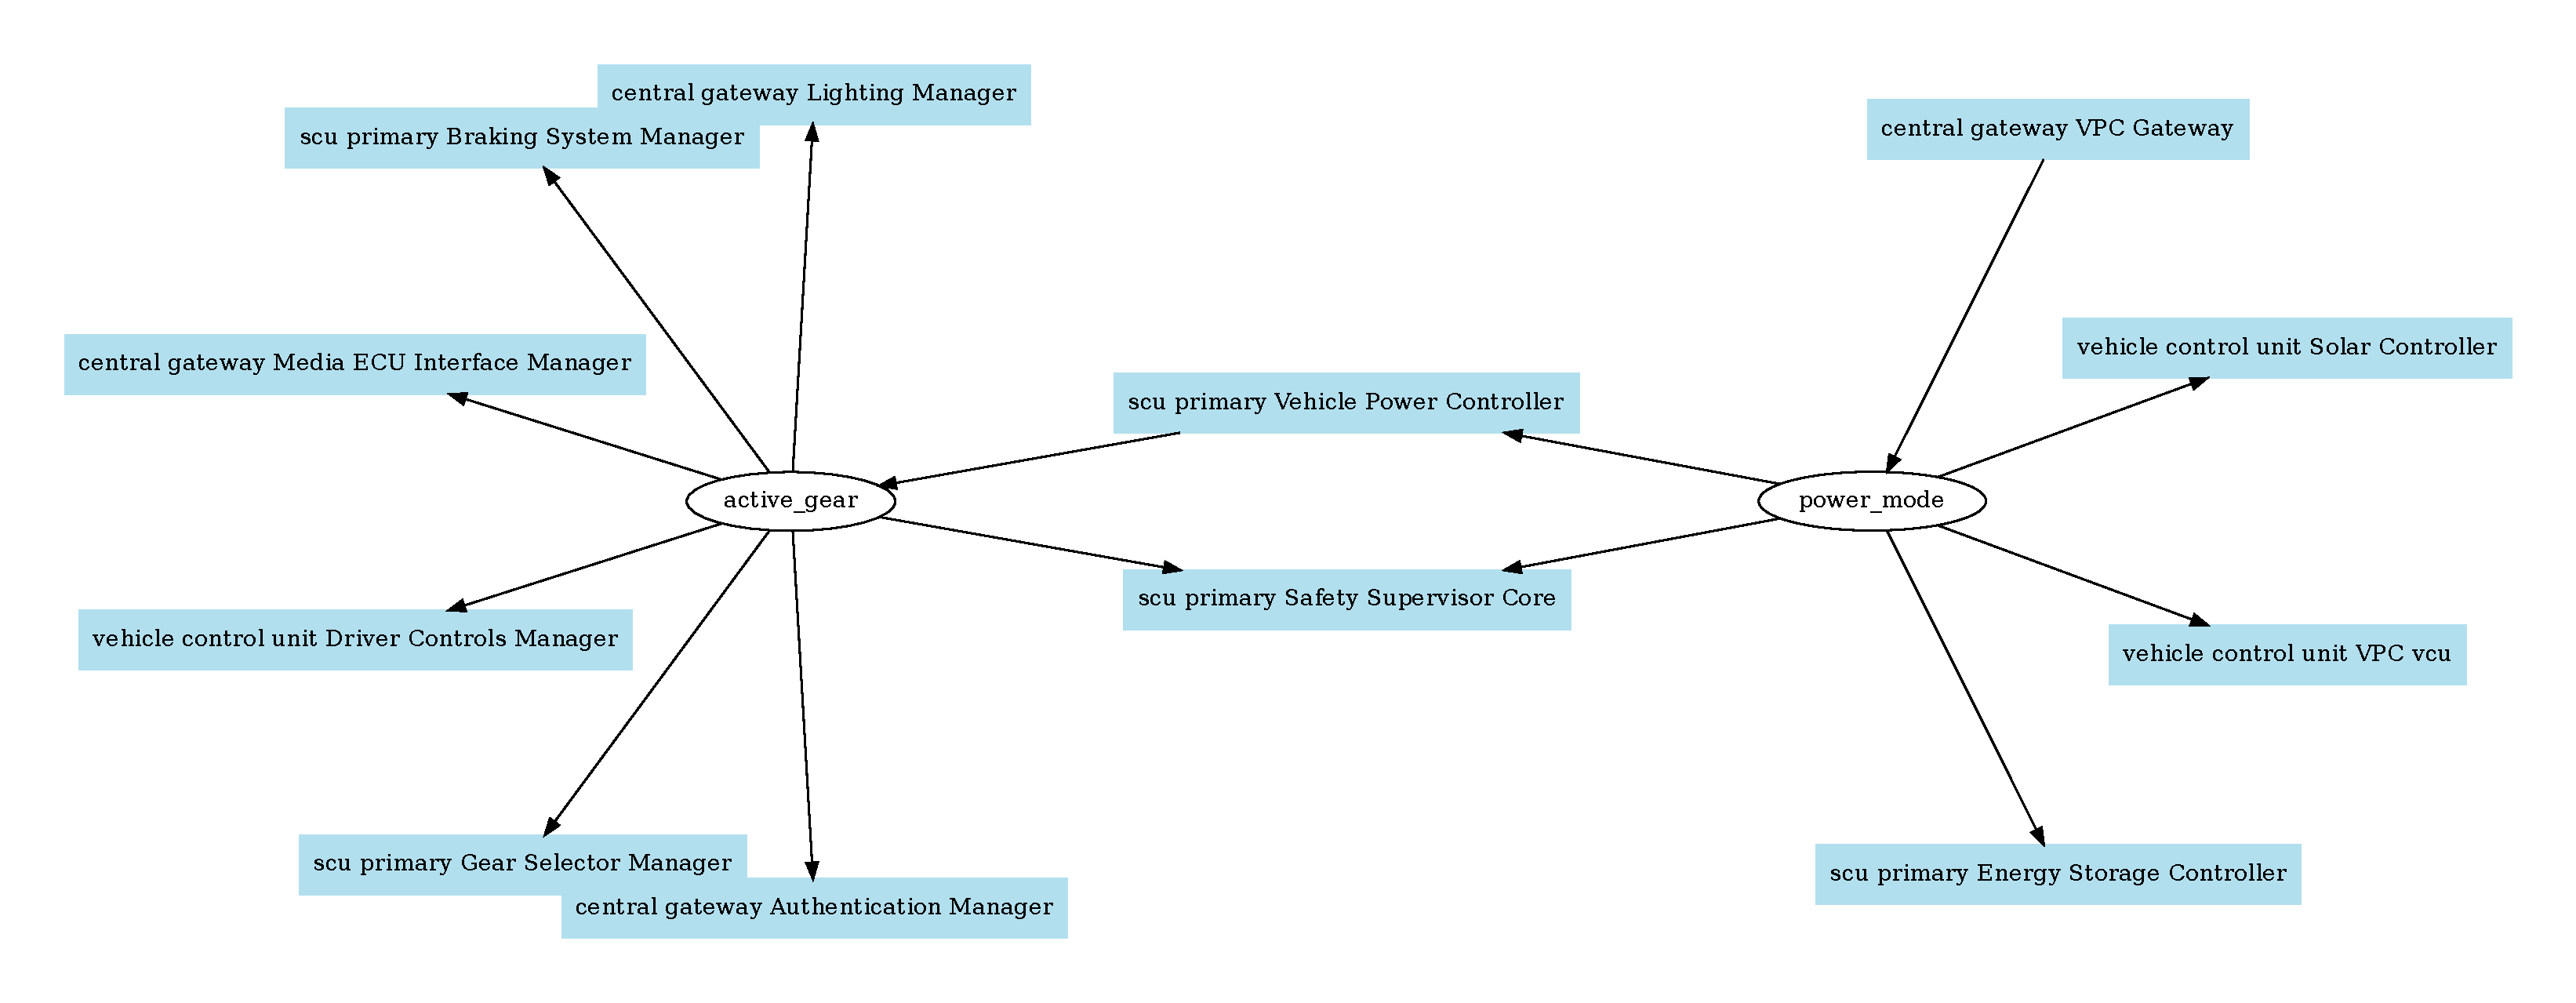
\includegraphics[width=\textwidth]{images/interface_overview.pdf}
    \caption{Interface overview for two signals in graphical form}
    \label{fig:interface_overview}
\end{figure}

\paragraph{Parametrizable end nodes}
The network traffic to and from \textit{parametrizable end nodes} is described in special deployment files called DBC files for CAN networks and LDF files for LIN networks. These are industry standards describing the messages that can be found on a network. For each message the content is described in terms of signals and how the raw bytes transmitted on the network map to a signal value. For example a signal \textit{brake pedal position} describing a numerical value has a certain data type (single precision floating point, 16-bit signed integer, 32-bit unsigned integer), but the numerical value can be also scaled and offset to represent the real value. The DBC and LDF standards describe how a set of received bytes can be reinterpreted as the original signal and how a measured value must be transformed in a set of bytes to transmit. 

In order to get the data flow to and from \textit{parametrizable end nodes} the LDF and DBC files are necessary as they describe which signals are communicated. Unfortunately these files do not always describe the source and destination of a signal, nor do they accurately describe the transmission rate, nor is it known which runnable from the \textit{programmable end nodes} consumes/produces the signal. This information is not available in a central and easily machine-readable format. A possible solution for partially retrieving this information is through static analysis of the \textit{programmable end node} software. The reception and transmission of the signals using the CAN and LIN busses happens by using a specific set of interfaces provided by the RTOS. By analysing call graphs of these interfaces the missing information could be retrieved. Some inaccuracies in the exact transmission rate of the signals might be introduced, but that is an acceptable risk given that we are using the data flow description as an input for simulating and evaluating various network configurations. A second solution would be to assume that each node on the bus consumes the transmitted data at exactly the rate at which it is transmitted. This would solve the lack of source and destination information but still misses the transmission rate. Additionally, it would introduce inaccuracies that could make the data flow description too pessimistic.

\paragraph{Aperiodic and non-real time data}
The description of dataflow by the various nodes so far serves as input/output of the various control applications in the vehicle e.g, cruise control or battery management, this type of traffic is (mostly) periodic and has a defined transmission rate. Data that is unrelated to the control systems is served on the same networks. For example applications such as software updates, remote diagnostics, logging of crucial signals all generate data that requires bandwidth on the network to reach the appropriate destination. To accommodate the complex requirements of these applications a transport layer is used to allow transmitting data packets with a data size that is larger than the maximum data size of a CAN frame. The chosen protocol is ISO~15765, known as ISO-TP, which acts as the network and transport layer in the OSI model.

The Telematics Control Unit (TCU) regularly checks if software updates are available, when an update is initiated the TCU transmits the update using ISO-TP to the end node that is updated. Because the TCU only has a direct CAN connection with the Central Gateway the update stream must be bridged by the Central Gateway to the correct CAN bus. When the to be updated end node has no direct connection with the Central Gateway, such as the inverters (Table~\ref{tab:networks}), the stream must be bridged again in this example by the Safety Control Unit. Similarly, logging of crucial signals occurs in an online database. The data is collected by the \textit{programmable end nodes} and transmitted to the TCU using ISO-TP. 

When a vehicle has to be serviced a technician can connect to the diagnostics port and run diagnostics using the industry standard ISO~14229 - Unified Diagnostic Services (UDS). UDS is a communication protocol specifically designed for diagnostics in vehicles. It allows technicians to read error codes of all the nodes in the network, perform tests and configure certain parameters. UDS uses ISO-TP as the transport layer, as the diagnostics port is connected to the Central Gateway bridging of the UDS messages occurs similarly to the software update stream when an end node is not directly connected to the Central Gateway.

Further investigation is necessary to understand which nodes generate aperiodic and non-real time data and what the underlying processes are that trigger this data to be transmitted. It is likely that certain dataflows only occur in specific use-cases, for example the diagnostics data will (probably) only occur when a service technician connects hardware to the diagnostics port and reads the status of the vehicle hardware. While other data streams can occur regularly during normal use of the vehicle, such as logging of specific signals in the cloud.

As shown previously the vehicle has several Ethernet networks. The inverters contain many internal signals which need to be sampled or change at high speeds (in the kHz range) to operate correctly e.g., current and voltage measurements. This is too much data to transmit over a CAN bus and can be irrelevant for other applications connected to the CAN bus. Hence, this data is transmitted over the Ethernet network such that during development and testing accurate information is available. The inverter Ethernet interfaces are strictly used for testing and debugging purposes only, nevertheless this is an interesting use case to consider during the design of a TSN based in-vehicle network.
\clearpage
\subsection{Discrete Event Simulation in \omnet}
\label{sec:omnetpp}
Since most relevant literature we wish to build upon uses \omnet as their discrete event simulation framework some experiments were performed. The first goal of the experiments is to create a working installation of \omnet and create a development environment in which the proposed solution can be developed. The second goal is to get acquainted with the modelling language and framework. Lastly the experiments validate that the framework is suitable for performing experiments involving random processes.

After installing \omnet and creating a development environment the \omnet tutorial~\cite{omnettutorial} was followed. This tutorial consists of 18 exercises showing the different aspects of the NED language and framework. To further study the framework and asses the suitability of \omnet for experiments of random processes an assignment from the Embedded Systems course 2IMN25 - Quantitative Evaluation of Embedded Systems is performed again. During the course a theoretical model for the expected steady-state distribution of the number of items in an $M/M/1/K$ queue was made, let $x$ be the number of items in the system, $k$ the maximum number of items in the system, $\lambda$ the arrival rate of items and $\mu$ the service rate of the items, then for $0 \leq x\leq k$ the probability of finding $x$ items in the system is described using Equation~\ref{eq:mm1k}. 
\begin{equation}
    \label{eq:mm1k}
p_\infty (x) = \left(\frac{\lambda}{\mu}\right)^x\cdot\frac{1-\frac{\lambda}{\mu}}{1-\left(\frac{\lambda}{\mu}\right)^{k+1}}
\end{equation}

A model of an $M/M/1/K$ queueing system was made in \omnet which is visualized in Figure~\ref{fig:mm1k_sim}. The system consists of an \textit{entityGenerator} which creates items with an intergeneration time that is drawn from an exponential distribution with a configurable rate $\lambda$. The generated items are then stored in a \textit{queue} of configurable size $K$. The \textit{sink} component takes an item from the \textit{queue} and takes execution time to handle the item before discarding it. The execution time is also drawn from an exponential distribution with a configurable rate $\mu$. An experiment is set up in which we log the queue occupancy in the steady state, \omnet is configured to automatically log the queue occupancy, run a simulation for 800000 s of simulated time and discard the data from the warm-up period of 300000 seconds of simulated time. Because the queue occupancy data points from a single simulation are not independent of each other \omnet is configured to repeat the simulation 50 times with different seed values for the random distributions.

\begin{figure}[htbp]
    \centering
    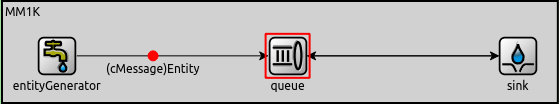
\includegraphics[width=\textwidth]{images/MM1K_sim.png}
    \caption{Visual view of an MM1K queue model in \omnet}
    \label{fig:mm1k_sim}
\end{figure}

The resulting data points are analysed with a python script in which we calculate the probability to find a certain queue occupancy in the simulation, with a 95\% confidence interval. The result of the simulation as well as the theoretical pdf are shown in Figure~\ref{fig:mm1k_sim}. The theoretical pdf falls inside the 95\% confidence interval for every queue occupancy, from this we conclude that the framework is able to properly simulate a random process.

\begin{figure}[htbp]
    \centering
    \includegraphics[width=\textwidth]{images/MM1k_analysis.png}
    \caption{Comparison of MM1K queue occupancy between simulation and theoretical analysis}
    \label{fig:MM1K_analysis}
\end{figure}
\todo{Pitfall in \omnet is manual memory management of events, can cause memory leaks}
\todo{write about logical modelling}

\begin{figure}[htb]
    \centering
    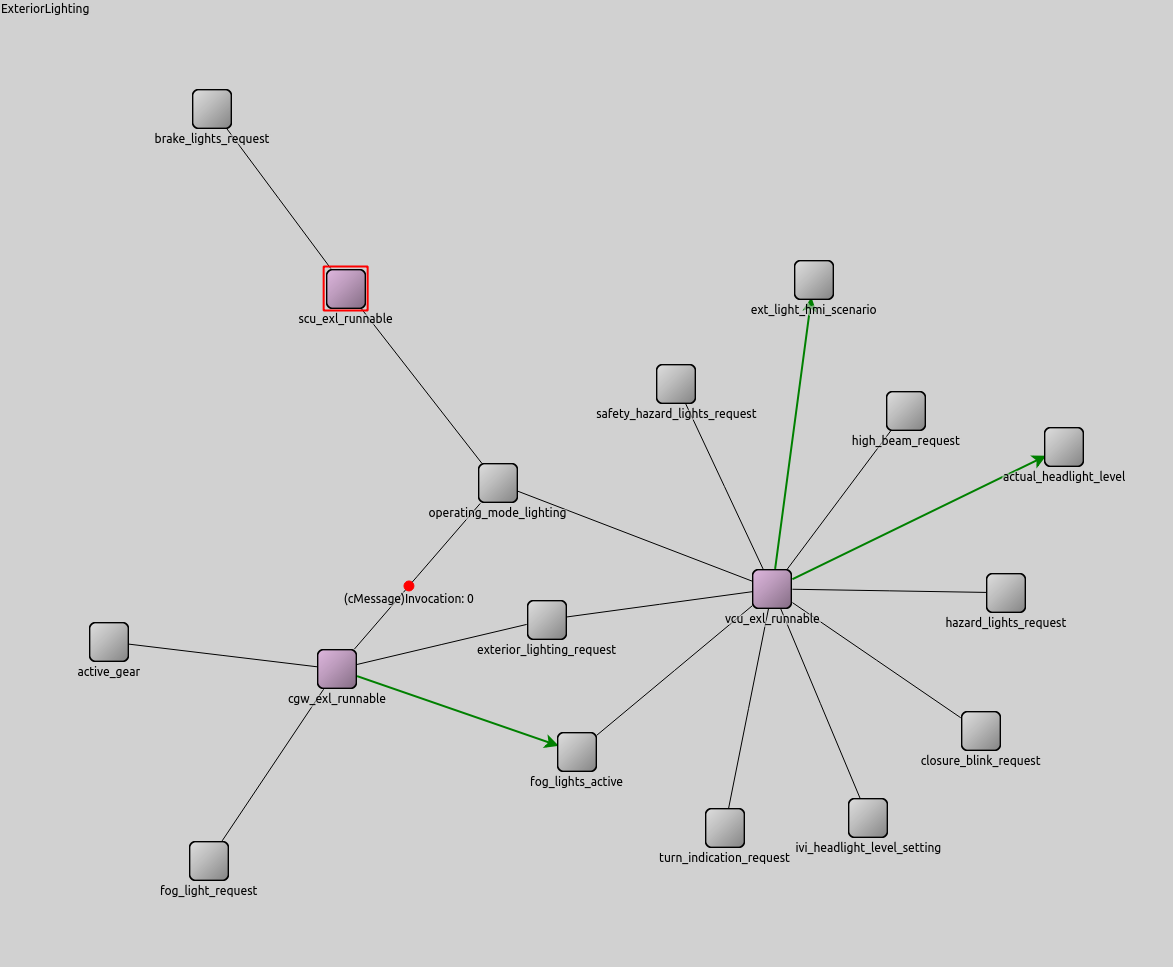
\includegraphics[width=\textwidth]{images/logical_sim.png}
    \caption{Modelling signal transmission of the logical architecture in \omnet}
    \label{fig:logical_sim}
\end{figure}

\newpage